\documentclass{abnt} 

%Arquivo com os principais pacotes usados e suas descrições.

%%%%%%%%%%%%%%%%%%%%%%%%%%%%%%%%%%%%%%%%%
% 			Idiomas e Acentos			%
%%%%%%%%%%%%%%%%%%%%%%%%%%%%%%%%%%%%%%%%%
\usepackage[brazil]{babel} % Habilita o uso do idioma português do brasil (PT-BR).
\usepackage[T1]{fontenc} 
%\usepackage{fontspec} % Habilita maior variedade de acentos. Pode ser necessario adicionar outros pacotes.
\usepackage{lmodern} % Habilita o uso da font Latin Modern.


%%%%%%%%%%%%%%%%%%%%%%%%%%%%%%%%%%%%%%%%%
% 				TABELAS					%
%%%%%%%%%%%%%%%%%%%%%%%%%%%%%%%%%%%%%%%%%
\usepackage{tabulary} % Cria tabelas mais facilmente.
\usepackage{booktabs} % Melhora o visual das tabelas.
\usepackage[table]{xcolor} % Pacote de cor pra as tabelas.
\usepackage{caption} % Melhora as legendas de imagens, tabela etc.

%%%%%%%%%%%%%%%%%%%%%%%%%%%%%%%%%%%%%%%%%
% 				IMAGENS					%
%%%%%%%%%%%%%%%%%%%%%%%%%%%%%%%%%%%%%%%%%
\usepackage{graphicx} % Facilita a inserção de imagens.


%%%%%%%%%%%%%%%%%%%%%%%%%%%%%%%%%%%%%%%%%
% 			CÓDIGO FONTE				%
%%%%%%%%%%%%%%%%%%%%%%%%%%%%%%%%%%%%%%%%%

%Documentação de código fonte.
\usepackage{listings}


%%%%%%%%%%%%%%%%%%%%%%%%%%%%%%%%%%%%%%%%%
% 	Símbolos e Caracteres Matemáticos	%
%%%%%%%%%%%%%%%%%%%%%%%%%%%%%%%%%%%%%%%%%
\usepackage{amsmath}
\usepackage{amssymb}
\usepackage{amsfonts}
\usepackage{mathspec} %Habilita o uso das fontes e dos caracteres matematicos.


%%%%%%%%%%%%%%%%%%%%%%%%%%%%%%%%%%%%%%%%%
%				ABNT					%
%%%%%%%%%%%%%%%%%%%%%%%%%%%%%%%%%%%%%%%%%
\usepackage[hidelinks] {hyperref} % LINK

\usepackage[alf, abnt-etal-cite=2]{abntcite} % Ordena as referencias em ordem alfabética.
\usepackage{url} %Facilita o uso de url. Pode-se usar o comando \url{...}.


%%%%%%%%%%%%%%%%%%%%%%%%%%%%%%%%%%%%%%%%%
% 			Configurações				%
%%%%%%%%%%%%%%%%%%%%%%%%%%%%%%%%%%%%%%%%%
\captionsetup{justification=centering,labelfont=bf} %Formata a legenda das figuras.
%\graphicspath{{../imgs/}} %Define o diretorio padrão para buscar as imagens da apresentação.  
%\setromanfont[Ligatures=TeX]{Crimson}
%\defaultfontfeatures{Scale=MatchLowercase, Mapping=tex-tex}

%%%%%%%%%%%%%%%%%%%%%%%%%%%%%%%%%%%%%%%%%
%				BEAMER					%
%%%%%%%%%%%%%%%%%%%%%%%%%%%%%%%%%%%%%%%%%
%Define algumas configurações que serão validas para todo o documento.  
%\setbeamertemplate{section in toc}[sections numbered]
%\setbeamertemplate{subsection in toc}[subsections numbered]
%\setbeamertemplate{background canvas}[vertical shading][bottom=blue!3,top=blue!7]
%\setbeamertemplate{caption}[numbered]

\usepackage{babel}
\usepackage{verbatim}
\usepackage{lscape}
\usepackage{rotating}

%%%%% Dados para criação da capa e folha de rosto %%%%
\autor{Victor Hugo Carlquist da Silva}
\titulo{Desenvolvimento de um Algoritmo Genético Híbrido para a solução do problema dos Múltiplos Caixeiros Viajantes (\textit{mTSP})}
\orientador{Prof. Me. André Malvezzi Lopes}
\coorientador{Prof. Dr. Silvio Alexandre de Araujo}
\comentario{Trabalho de Conclusão de Curso em Tecnologia em Análise e Desenvolvimento de Sistemas.}
\instituicao{Instituto Federal de Educação, Ciência e Tecnologia de São Paulo -- \textit{campus} Campos do Jordão}
\local{Campos do Jordão, SP}
\data{\today}

\definecolor{blues}{rgb}{0.13,0.13,1}
\definecolor{greens}{rgb}{0,0.5,0}
\definecolor{reds}{rgb}{0.9,0,0}

\lstset{language=C++,
basicstyle = \ttfamily\tiny, % Tamanho da fonte do código
numbers = left, % Posição da numeração das linhas
numberstyle = \tiny\color{blue}, % Estilo da numeração de linhas
stepnumber = 0, % Numeração das linhas ocorre a cada quantas linhas?
numbersep = 10pt, % Distância entre a numeração das linhas e o código
backgroundcolor = \color{white}, % Cor de fundo
showspaces = false, % Exibe espaços com um sublinhado
showstringspaces = false, % Sublinha espaços em Strings
showtabs = false, % Exibe tabulação com um sublinhado
frame = trbl, % Envolve o código com uma moldura, pode ser single ou trBL
rulecolor = \color{black}, % Cor da moldura
tabsize = 2, % Configura tabulação em x espaços
captionpos = b, % Posição do título pode ser t (top) ou b (bottom)
breaklines = true, % Configura quebra de linha automática
breakatwhitespace= false, % Configura quebra de linha
%title = \lstname, % Exibe o nome do arquivo incluido
%caption = \lstname, % Também é possível usar caption no lugar de title
keywordstyle = \color{blues}, % Estilo das palavras chaves
commentstyle = \color{greens}, % Estilo dos Comentários
stringstyle = \color{reds}, % Estilo de Strings
escapeinside = {\%*}{*)}, % Permite adicionar comandos LaTeX dentro do seu código
morekeywords     ={*,USE,GO} % Se quiser adicionar mais palavras-chave
}

\begin{document}
	%\bibliographystyle{plain}
	% Para utilizar o formato padrão de capa da ABNT, substituí o comando \maketitle pelo comando \capa.

	\capa
	
	\folhaderosto
	
	\begin{folhadeaprovacao}
	
	\setlength{\ABNTsignthickness}{1pt}
	\begin{center} 
		VICTOR HUGO CARLQUIST DA SILVA \\~\\
		\large{\textbf{DESENVOLVIMENTO DE UM ALGORITMO GENÉTICO HÍBRIDO PARA A SOLUÇÃO DO PROBLEMA DOS MÚLTIPLOS CAIXEIROS VIAJANTES (\textit{mTSP})}}
	\end{center}
	Trabalho de Conclusão de Curso em Tecnologia em Análise e Desenvolvimento de Sistemas.
	
	\begin{center}
		~\\~
		\textbf{BANCA EXAMINADORA}\\
		10 de junho de 2014\\
	\assinatura*{\textbf{Prof. Alisson Ribeiro}\\ Instituto Federal de Educação, Ciência e Tecnologia}\\
	\assinatura*{\textbf{Profª. Dra. Thalita Biazzuz Veronese}\\ Instituto Federal de Educação, Ciência e Tecnologia}\\
	\assinatura*{\textbf{Prof. Paulo Giovani de Faria Zeferino}\\Instituto Federal de Educação, Ciência e Tecnologia}\\~\\~\\
	
	\textbf{LOCAL}\\
	
	Instituto Federal de Educação, Ciência e Tecnologia de São Paulo -- IFSP\\ \textit{Campus} Campos do Jordão \\ Campos do Jordão, SP
	\end{center}
	\end{folhadeaprovacao}
	
	\sumario 

	%\listadetabelas
	
	\listadefiguras
	
	\begin{resumo}
		A alta complexidade para definir a melhor rota para diversos veículos estimula o desenvolvimento de novos algoritmos computacionais para resolver este problema. Este problema pode ser definido como o problema dos múltiplos caixeiros viajantes (\textit{Multiple Traveling Salesman Problem} (MTSP)). Portanto, foi proposto um algoritmo Algoritmo Genético otimizado, dividindo o espaço dos objetivos para otimizar o cruzamento dos indivíduos, diminuindo assim o número de gerações necessárias para conseguir uma rota ótimo, ou quase ótima.
		%O resultado deste novo algoritmo será comparado com o Algoritmo Genético ``tradicional''

	\end{resumo}

	\begin{abstract}
		The high complexity to define the best route for multiple vehicles motivate a development for a new algorithm to solve this problem. This problem is known as multiple Traveling Salesman Problem (\textit{mTSP}). It was created a hybrid algorithm using Genetic Algorithm with NN Algorithm. Executing and analysing results of the software, it shows very efficient to solve the mTSP.  
	\end{abstract}

	\chapter{Introdução}
		
		A importância do transporte veicular nos dias de hoje causa impactos positivos e negativos 
		na sociedade e no meio ambiente, principalmente na economia mundial \cite{meioAmbiente}. 
		
		Apesar de agilizar o transporte de pessoas e  de mercadorias, 
		os veículos também geram despesas com combustível e manutenção, entre outros fatores. 
		Se um veículo percorrer uma menor rota, a empresa diminui custos, com, por exemplo, 
		combustível, manutenção e tempo de entrega.

		O crescimento das cidades e da complexidade rodoviária dificulta a análise da melhor rota a se percorrer. Esse problema tende a ficar mais complexo conforme aumenta a quantidade de veículos que a empresa possui. Com isso, surge a necessidade de criar 
		\textit{softwares} cada vez mais robustos que resolvam o problema de roteirização de veículos, encontrando o melhor caminho para os veículos percorrer, realizando suas entregas nestes pontos já pré-estabelecidos.


	\chapter{Metodologia}

		O objetivo deste trabalho é desenvolver um novo algoritmo, ou otimizar um algoritmo, para que encontrasse a rota ótima\footnote{Quando a rota gerada por um algoritmo é o menor caminho possível, essa rota é considerada uma ``rota ótima''.} ou quase ótima, para o problema dos múltiplos caixeiros viajantes, consumindo menos recurso computacional, mais especificamente o tempo de execução. 

		Antes de se iniciar o desenvolvimento do algoritmo híbrido, foi realizado o levantamento bibliográfico sobre o assunto e debatido como otimiza-lo com o orientador do projeto.

		Foi utilizado a base de testes TSPLIB desenvolvida para o Problema do Caixeiro Viajante (TSP) \footnote{Disponível em \url{http://www.math.uwaterloo.ca/tsp/world/countries.html}}, já que não foi possível encontrar uma base de testes específica para o MTSP. Esta base de testes foi utilizada como referência para medir o desempenho das rotas e o tempo de execução do algoritmo híbrido desenvolvido\footnote{O TSPLIB se baseia em informações geográficas do \textit{National Imagery and Mapping Agency}} \cite{tsplib}.

		Para exemplificar, foi escolhido um teste da base TSPLIB que já possuí resultados de outros algoritmos, como a distância encontrada e o tempo que o algoritmo levou para entrar a rota. O teste foi submetido ao algoritmo híbrido os resultados que ele gerou foram comparados com os resultados da base TSPLIB.

		Após esses testes foram utilizados diversas configurações de cenário, modificando os parâmetros do Algoritmo Genético, que serão explicado neste trabalho, comparando o tamanho das rotas e o tempo de execução do Algoritmo Genético ``tradicional'' com o algoritmo híbrido para verificar a eficiência e eficacia do algoritmo híbrido. 

	
	\chapter{Problema do Caixeiro Viajante - TSP}
		O problema do Caixeiro Viajante (\textit{Traveling Salesman Problem} - TSP) consiste em estabelecer uma rota para um \textbf{único} caixeiro, passando por cada vértice do grafo apenas uma vez e retorne ao vértice de partida. O número de rotas possíveis pode ser expressa por $(n-1)!$, sendo $n$ o número de pontos.
		O problema TSP é classificado como \textit{NP-Hard}\cite{0015-pdf}, ou seja, não existe algoritmo com limitação polinominal capaz de resolvê-lo \cite{0010-pdf}. 
		
		Este problema pode ser formulado da seguinte forma:
		\begin{equation}
 		   	min\sum_{i=1}^{n} \sum_{j=1}^{n} c_{ij} x_{ij}
		\end{equation}
		
		então		
		\begin{equation}
			\label{form}
 		   	\sum_{i=1}^{n} x_{ij} = 1 \quad j=1,\dots,n
		\end{equation}
		\begin{equation}
			\label{form-1}
 		   	\sum_{j=1}^{n} x_{ij} = 1 \quad i=1,\dots,n
		\end{equation}
		\begin{equation}
		\label{form-2}
 		   	\{(i,j)|i,j=2,\dots,n; x_{ij}=1\} ~\text{não contém sub-rotas,}
		\end{equation}
		
		\begin{equation}
		\label{form-3}
 		   	x_{ij} \in \{0,1\}\forall i,j=1,\dots,n
		\end{equation}
		
			
		Para um grafo  $G=(V,A)$, onde $V$ é o conjunto de vértices e $A$  é o conjunto de arestas, sendo $C = (C_{ij})$ a matriz que corresponde ao custo associado com $A$. A matriz $C$ é simétrica caso $c_{ij}=c_{ji},\forall(i,j) \in A$ e assimétrica caso contrário. A variável $x_{ij}$ é binária, usada para indicar se a aresta foi usada na rota. As equações \ref{form} e \ref{form-1} criam uma restrição, para que haja um caminho de entrada e um caminho de saída para cada cidade. Já a equação \ref{form-2} previne sub-rotas, ou seja, não permite um grafo desconexo \cite{dissertation}
	
	\section{Problema dos Múltiplos Caixeiros Viajantes}

		O problema dos Múltiplos Caixeiros Viajantes (\textit{Multiple Traveling Salesman Problem - mTSP}) é uma extensão do TSP citado na sessão anterior.
		Neste problemas há mais de um caixeiro que precisar visitar um conjunto de vértices, sendo que não é permitido um caixeiro visitar uma vértice que o outro caixeiro já visitou, estabelecendo várias rotas, uma para cada caixeiro viajante.

		Sendo assim, o Problema dos Múltiplos Caixeiros Viajantes torna-se  mais complexo conforme o número de caixeiros aumenta, porque é necessário distribuir os vértices (cidades) da melhor possível para cada caixeiro, tentando reduzir o tamanho das rotas. 

		O algoritmo híbrido desenvolvido leva em consideração o tamanho da rota global, não importando o tamanho da rota de cada caixeiro, ou seja, o algoritmo híbrido não tenta igualar o tamanho das rotas entre os caixeiros  \cite{dissertation}.
	
	\chapter{Algoritmos genéticos}

		Segundo \citeonline{0008-pdf}, os Algoritmos Genéticos (AGs) são técnicas de procura e otimização baseadas em mecanismos de seleção natural. 

		Nas décadas de 60 e 70, John Holland e seus colegas da Universidade de Michigan criaram modelos para estudar o processo de adaptação dos seres vivos. Holland realizou diversas pesquisas e em 1975 publicou o seu livro intitulado \textit{Adaptation in Natural and Artificial System} \cite{john}. Hoje, este livro é considerado um dos mais importantes sobre Algoritmos Genéticos \cite{0001-pdf}.

		No Algoritmo Genético, o cromossomo, também chamado de indivíduo, é representado por um conjunto de genes que armazena uma possível solução de um problema. Cada gene possui um valor que representa um vértice do grafo, sendo assim, os indivíduos são cruzados gerando novos indivíduos com sequência de genes (vértices) diferentes. Conforme a população cresce, surgem indivíduos cada vez mais aptos, ou seja, armazenam em seus cromossomos uma solução para o problema cada vez melhor, sendo que um deles será o mais apto, contendo no seu cromossomo a solução do problema, portanto, este indivíduo terá a melhor sequência de vértices, entre os indivíduos da população, pelo qual o caixeiro deverá passar.

		O Algoritmo Genético possui alguns parâmetros importantes para configurar a evolução dos indivíduos, por exemplo, o tamanho da população, que indica quantos indivíduos existirão para realizar o cruzamento. Se o número da população for pequena deixará as rotas ruins (muito grandes), pois terá um pequeno conjunto para a busca da solução do problema. Já uma população muito grande pode afetar o desempenho do algoritmo, também  existe a \textbf{taxa de mutação}, que define as chances de um cromossomo sofrer mutação. Uma alta taxa de mutação irá deixar o algoritmo aleatório, mas com uma baixa taxa previne que os indivíduos sejam sempre os mesmos. É preciso salientar que estes parâmetros são pertinente ao algoritmo e não ao modelo matemático.

		\section{Operadores de cruzamento}

			Os operadores de cruzamento definem como ocorrerá o cruzamento entre dois indivíduos, ou seja, como será a feita a troca de uma sequência de genes entre dois indivíduos, gerando novos indivíduos na população \cite{0012-pdf}.

			Neste trabalho foi utilizado o Cruzamento de Mapeamento Parcial, que foi utilizado no algoritmo híbrido.

		\subsection{Cruzamento de Mapeamento Parcial - PMX} 
			\label{Spmx}
			O operador de Cruzamento de Mapeamento Parcial (\textit{Partially-mapped crossover} - PMX)  seleciona e copia três genes do pai para um filho e completa o restante do cromossomo com os genes do outro pai, como a \textbf{figura~\ref{pmx}} demonstra.

			\begin{figure}[h]
				\centering
		        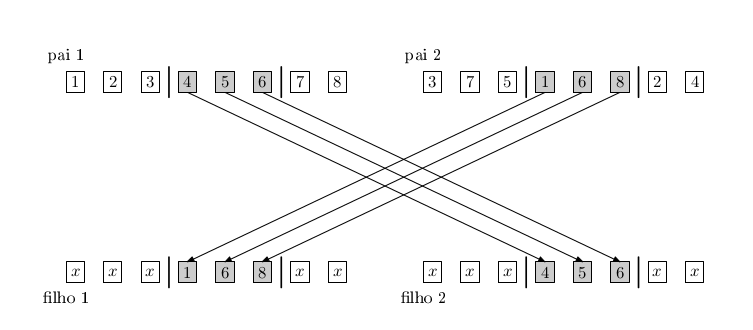
\includegraphics[width = 14cm,keepaspectratio]{img/pmx.png}
		        \caption{PMX - cruzamento}
		        \caption*{Fonte:\cite{0012-pdf}.}
		        \label{pmx}
	   		\end{figure}

	   		Caso o cromossomo já possua o mesmo número, é escolhido outro número com o mesmo índice do pai que não esteja no cromossomo:
	   		\begin{figure}[h]
				\centering
		        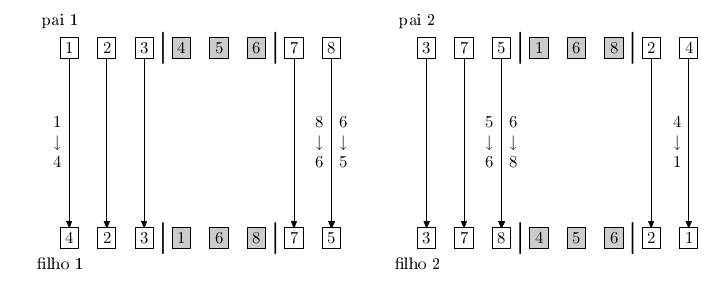
\includegraphics[width = 14cm,keepaspectratio]{img/pmx2.png}
		        \caption{PMX - preenchimento}
		        \caption*{Fonte:\cite{0012-pdf}.}
		        \label{pmx2}
	   		\end{figure}

	   		Por exemplo, como o ``filho 1'' já possui o valor 1, então é pesquisado qual a posição que o valor 1 está neste vetor, no caso da \textbf{figura~\ref{pmx2}} o valor 1 está na posição 4, então o valor na posição 4 do vetor do ``pai 1'' é copiado para a posição 1 do vetor ``filho 1''. No outro exemplo na mesma figura, na terceira posição do vetor do ``filho 2'',  o número 5 já existe na posição 5, sendo assim, o valor que está na posição 5 no vetor ``pai 2'' é o valor 6, mas este valor também existe do vetor ``filho 2'', portanto é pesquisado a posição do valor 6 no vetor ``filho 2'', que neste caso é a posição 6, então copia-se o valor 8 que está na posição 6 do vetor ``pai 2'' para a terceira posição do vetor ``filho 2''. 
	   		Este processo descrito acima é repetido para todos os outros elementos vazios\footnote{Os valores vazios são representados pelos caracteres ``x'' na \textbf{figura~\ref{pmx}}} dos filhos.
	   		  
		\section{Operador de mutação}
			\label{Sem}
			O operador de mutação define como será realizada a mutação de um cromossomo, impedindo que o programa sempre gere os mesmos indivíduos (cromossomos) \cite{0012-pdf}.

			Foi implementado no algoritmo proposto o operador de mutação por troca \textit{exchange mutation} (EM). Ele seleciona dois genes, aleatoriamente, do cromossomo e os troca de posição.

		\section{Algoritmo Genético Híbrido}

			Os Algoritmos  Genéticos possuem o objetivo de serem robustos, ou seja, são eficientes nas soluções de problemas com complexidade \textit{NP-HARD}, mas, estes algoritmos têm dificuldade em encontrar o caminho ótimo. Para solucionar esse problema foram criados os Algoritmos Genéticos Híbridos.

			Os Algoritmos Genéticos Híbridos consistem em utilizar um outro algoritmo em conjunto com o Algoritmo Genético, produzindo algoritmos eficientes na prática \cite{TravelingTheory}.
			
		\chapter{Estado da Arte}
		
			Existem diversos trabalhos sobre a utilização de Algoritmos Genéticos na resolução do problema do TSP.
			Segundo \citeonline{0002-pdf}, implementaram uma solução para este problema, os Algoritmos Genéticos não são eficientes 
			na resolução do TSP em comparação com métodos algoritmos determinísticos. Neste trabalho o Algoritmo Genético foi executado em um período de tempo maior e não encontrou a solução ótima em comparação com algoritmos determinísticos.

			A solução apresentada por \citeonline{0006-pdf} propõe resolver os problemas de roteirização de 
			veículos com entregas fracionadas, problema clássico de roteirização de veículos e com 
			frota heterogênea criando o algoritmo de roteirização de veículos com frota heterogênea, 
			restrições de janelas de tempo e entregas fracionadas(\textit{Heterogeneous Fleet Vehicle 
			Routing Problem with Time Windows and Split Deliveries} (HFVRPTWSD)) utilizando Algoritmo 
			Genético (AG).

			Na proposta  apresentada por \citeonline{0011-pdf} para a resolução do \textit{mTSP} com um depósito, foi criado um único cromossomo utilizando o método \textit{two-part}, que será explicado na próxima seção. Este método mostrou-se muito eficiente.

			\citeonline{0005-pdf}  mostra que é possível calcular as rotas de múltiplos veículos utilizando AG para igualar o tempo 
			de espera de encomendas de clientes, sendo que a variável ``menor tempo da rota'' não é levada em consideração.


		\chapter{Algoritmo \textit{Nearest-Neighbor} (NN)}

			O Algoritmo \textit{Nearest-Neighbor} (NN) é classificado como um algoritmo guloso\footnote{Um algoritmo guloso preza pela menor rota localmente, sem se preocupar com o desempenho da rota globalmente}.

			O NN é um algoritmo simples implementação, sua única tarefa é verificar selecionar um ponto e verificar quais pontos ao seu redor esta mais próximo deste e coloca-lo como próximo ponto á ser visitado. Após esse passo é repetido o mesmo processo para este ponto escolhido. 

			O Algoritmo NN possuí possui uma alta complexidade, $O((n-1)!)$, pois faz a comparação com todos os pontos ainda não visitados, sendo inviável sua utilização para muitos pontos \cite{NN}.
	
		\chapter{Desenvolvimento}
		
		O Algoritmo Genético Híbrido proposto, utiliza os conceitos do Algoritmo Genético tradicional em conjunto com o algoritmo  \textit{Nearest-Neighbor} (NN).

		Foi necessário criar um Algoritmo Genético Híbrido porque após os primeiros teste utilizando apenas o Algoritmo Genético foi possível notar que o Algoritmo Genético não era eficiente, pois gerava rotas grandes (aproximadamente 72 vezes maior que a menor rota no TSPLIB). Para solucionar este problema, foi adicionado o algoritmo \textit{Nearest-Neighbor}. 

		%ISSO DEVERA MUDAR APOS A IMPLEMENTAÇÃO DE TODA A POPULAÇÃO FOR GERADA POR NN
		%ISSO DEVERA MUDAR APOS A IMPLEMENTAÇÃO DE TODA A POPULAÇÃO FOR GERADA POR NN
		%ISSO DEVERA MUDAR APOS A IMPLEMENTAÇÃO DE TODA A POPULAÇÃO FOR GERADA POR NN
		%ISSO DEVERA MUDAR APOS A IMPLEMENTAÇÃO DE TODA A POPULAÇÃO FOR GERADA POR NN
		%ISSO DEVERA MUDAR APOS A IMPLEMENTAÇÃO DE TODA A POPULAÇÃO FOR GERADA POR NN
		%ISSO DEVERA MUDAR APOS A IMPLEMENTAÇÃO DE TODA A POPULAÇÃO FOR GERADA POR NN
		%ISSO DEVERA MUDAR APOS A IMPLEMENTAÇÃO DE TODA A POPULAÇÃO FOR GERADA POR NN
		O algoritmo \textit{Nearest-Neighbor} é utilizado para gerar apenas um indivíduo na população inicial, os outros indivíduos são gerados aleatoriamente.
		
		\section {\textit{Nearest-Neighbor} alterado}

		Como já citado o Algoritmo NN possui uma alta complexidade. Para resolver este problema, o plano cartesiano foi dividido em 4 áreas de tamanhos iguais, sendo que o número de áreas pode ser alterado. 
		Com isso, pode-se aplicar o NN em cada area, sendo assim, os pontos de uma area não podem ser comparados com os pontos de outras areas reduzindo assim a complexidade para, na melhor hipótese, $(\frac{n}{k}-1)!k$, sendo $n$ o número total de pontos e $k$ o número de áreas e na pior hipótese $n!$. 
		
		O número de áreas sempre deve ser par, e o plano cartesiano sempre terá duas linhas, por exemplo, caso o número de áreas for definido em 8 partes, então a primeira linha do plano cartesiano terá 4 áreas de tamanhos iguais e a segundo linha também terá 4 áreas de tamanhos iguais totalizando 8 áreas.
		
		
		\section{Estrutura do cromossomo (indivíduo) - \textit{two-part}}
		
			O método utilizado para definir a estrutura do cromossomo do programa foi o \textit{two-part}.
			O \textit{two-part} consistem em dividir o cromossomo em duas partes, uma parte armazena as informações da rota e a outra a informação dos caixeiros. Considere o cromossomo a seguir:

			\begin{center}
				| 1 | 9 | 10 | 3 | 11 | 5 | 4 | 2 | 6 | 7 | 8 || 2 | 6  | 3 |
			\end{center}

			Os três últimos genes representam os caixeiros. Neste exemplo foi definido o ponto de partida como sendo o 0. Seguindo este raciocínio, o primeiro caixeiro terá que sair do ponto 0 e visitar dois pontos, ou seja, os pontos 1 e 9 e retornar ao ponto 0, já o segundo caixeiro terá que sair do ponto 0 e visitar seis pontos, os pontos 10, 3, 11, 5, 4 e 2 e retornar ao ponto 0 e o último caixeiro terá que sair do ponto 0 e visitar três pontos, os pontos 6,7 e 8 e retornar ao ponto 0. (\textbf{figura~\ref{two-part}}).

			\begin{figure}[h]
				\centering
		        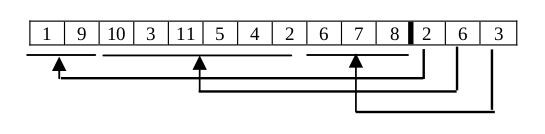
\includegraphics[width = 9cm,keepaspectratio]{img/two-part.png}
		        \caption{Cromossomo - \textit{two-part}}
		        \caption*{Fonte: \cite{0011-pdf}.}
		        \label{two-part}
	   		\end{figure}
	   	
	   	\section{Avaliação do Indivíduo (\textit{fitness})}

		Para cada novo indivíduo gerado, é calculado a distância dos pontos da rota, por meio da distância euclidiana,  de cada caixeiro e somando-as, gerando o tamanho total da rota, quanto menor este valor, melhor é o indivíduo.
				

		\section{Cruzamento}

			O programa proposto utiliza o operador de cruzamento PMX, descrito no capítulo (\ref{Spmx}). 
			
			A cada iteração é realizado um cruzamento, para isso é selecionado, aleatoriamente, dois cromossomos da população. No cruzamento é gerado dois novos indivíduos, esses indivíduos serão avalizados pela função \textit{fitness} e inseridos na população conforme sua avaliação.

		\section{Mutação}

			O programa proposto utiliza o operador de mutação EM (\textit{Exchange Mutation}), descrito no capítulo~\ref{Sem}. O indivíduo é escolhido aleatoriamente para receber a mutação.
			
						
		\section{Parâmetros}
		
		Segundo \citeonline{0001-pdf} os parâmetros são importantes para analisar o comportamento do algoritmo e ajustá-lo para suprir as necessidades do problema. 
		
		No algoritmo proposto foram implementados os seguintes parâmetros:
		 
			\begin{itemize}
				\item \textbf{MaxPopulation:} Define o número máximo da população; 
				\item \textbf{InitialPopulation:} Define a quantidade inicial de indivíduos dentro da população, as rotas destes indivíduos serão gerados aleatoriamente. Caso o parâmetro \textit{InitialPopulationWithNN} estiver ativado, um indivíduo será gerado utilizando o algoritmo NN;
				\item \textbf{InitialPopulationWithNN:} Se for igual a \textit{true} um indivíduo da população inicial será gerado utilizando o algoritmo NN;
				\item \textbf{MutationRouteItself:} Se for igual a \textit{true} a mutação ocorrerá dentro da rota de um caixeiro viajante, ou seja, os pontos da rota de um caixeiro não poderão ser trocadas com outros caixeiros. Se for igual a \textit{false} os pontos poderão ser trocados entre os caixeiros;
				\item \textbf{NNsizePart:} Define o tamanho da área que os pontos serão gerados, por exemplo, se está variável possuir o valor 100, então será criada um espaço 100x100;
				\item \textbf{NNnPart:} Define o número de áreas que o espaço será dividido para a utilização do algoritmo NN;
				\item \textbf{RateMutation:} Define a probabilidade de um indivíduo da população sofrer mutação;
				\item \textbf{RateGeneration:} Define a chance de adicionar ou substituir novos indivíduos na população, por exemplo, se o parâmetro \textit{MaxPopulation} for maior que o valor do parâmetro \textit{Initial Population}, então os dois novos indivíduos que serão gerados por meio do cruzamento terão chances de substituir um indivíduo da população, mesmo que o número máximo da população não tenha sido atingido, ou serão adicionados sem substituir nenhum indivíduo. Após a população atingir o número máximo permitido pelo parâmetro \textit{MaxPopulation}, apenas ocorrerá substituição dos piores indivíduos;
				\item \textbf{RateSalesmanMutation:} Define a probabilidade de mutação no número de pontos que cada caixeiro irá visitar, ou seja, irá afetar a segunda parte do cromossomo (\textit{two-part});
				\item \textbf{Generation:} Define o número de iterações que o programa realizará;
				\item \textbf{Deposit:} Define qual ponto será o depósito no qual os caixeiros irão sair;
				\item \textbf{Salesman:} Define o número de caixeiros viajantes;
				\item \textbf{SaveBetterChromo:} Se for igual a \textit{true}, o melhor indivíduo não poderá sofrer mutação;
			\end{itemize}
			
		\section{Desempenho}
		
		Para mensurar o desempenho do algoritmo foram realizados diversos teste com parâmetros diferentes, levando em consideração o tamanho da rota e o tempo de execução.
		
		O algoritmo foi implementado utilizando a linguagem C++ e os gráficos foram gerados pelo programa \textit{gnuplot}.
		O computador que executou os testes possuí processador Intel\textregistered Core\texttrademark ~i5 2,4Hz, 4GB de memória RAM.
		
		Foi gerado um cenário aleatoriamente com 600 pontos, executando 9000 gerações com 4 caixeiros,  para demonstrar o desempenho do Algoritmo Genético tradicional e o desempenho do Algoritmo Híbrido.
		

		\begin{figure}[h]
				\centering
		        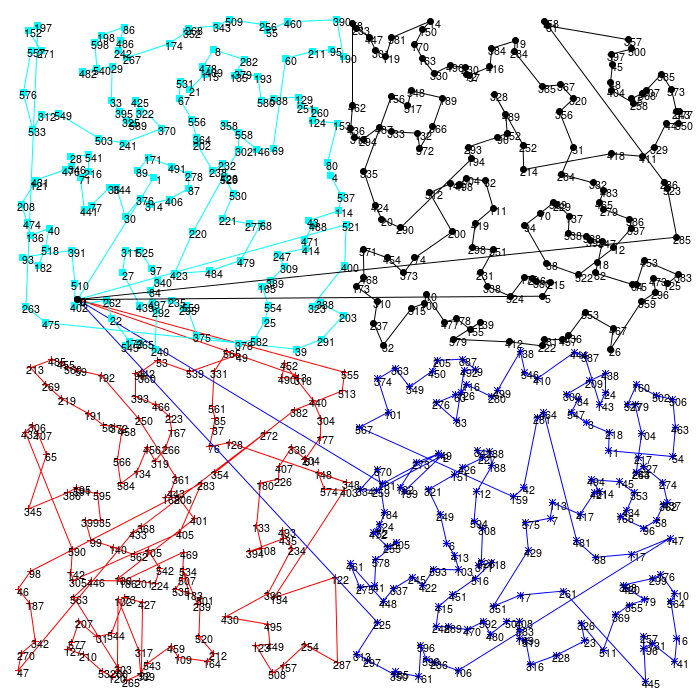
\includegraphics[width = 9cm,keepaspectratio]{img/ga-nn.png}
		        \caption{Resultado utilizando o algoritmo NN e AG - 4 caixeiros.}
		        \label{ga-nn}
	   		\end{figure}
		
		\begin{figure}[h]
				\centering
		        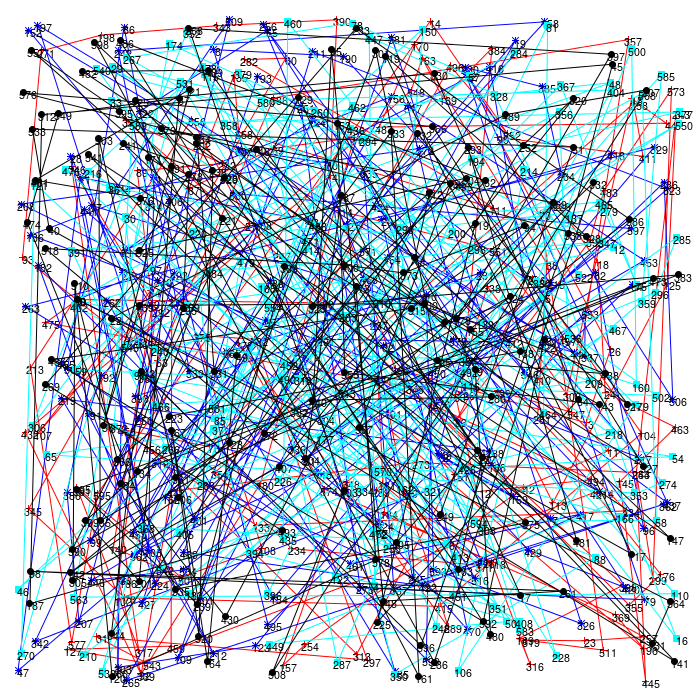
\includegraphics[width = 9cm,keepaspectratio]{img/ga-ale.png}
		        \caption{Resultado utilizando o AG tradicional com 4 caixeiros.}
		        \label{ga-ale}
	   	\end{figure}
	
	
		Utilizando este cenário foi executados os testes apresentados na \textbf{tabela~\ref{tst-01}}. Pode-se notar que utilizando algoritmo NN a distância da rota é bem reduzida se comparado ao algoritmo tradicional (Teste 4).  O algoritmo tradicional gerou uma rota com tamanho de 273.202km (\textbf{figura~\ref{ga-ale}}) e o Algoritmo Híbrido utilizando o \textit{Nearest-Neighbor} gerou uma rota com tamanho de 26.629,6km (\textbf{figura~\ref{ga-nn}}). 
		
		\begin{table}[htbp]
			\centering
			\begin{tabular}{|l|r|r|r|r|}
				
				\hline
				&Teste 1 &Teste 2 &Teste 3 &Teste 4 \\
				\hline
				MaxPopulation & 100 & 10 & 10 & 10\\ \hline
				Initial Population & 10 & 10 & 10 & 10\\ \hline
				InitialPopulationWithNN & \multicolumn{1}{c|}{true} & \multicolumn{1}{c|}{true} & \multicolumn{1}{c|}{true} & \multicolumn{1}{c|}{false} \\ \hline
				MutationRouteitself & \multicolumn{1}{c|}{true} & \multicolumn{1}{c|}{true} & \multicolumn{1}{c|}{true} & \multicolumn{1}{c|}{true}\\ \hline
				NnsizePart & 1000 & 1000 & 1000 & 1000 \\ \hline
				Nnnpart & 4 & 4 & 4 & 4 \\ \hline
				RateMutation & 0,8 & 0,8 & 0,8 & 0,8 \\ \hline
				RateGeneration & 0,2 & 0,2 & 0,2 & 0,2 \\ \hline
				RateSalesmanMutation & 0 & 0 & 0 & 0 \\ \hline
				Generation & 9000 & 9000 & 10000 & 9000\\ \hline
				Deposit & 0 & 0 & 0 & 0 \\ \hline
				Salesman & 4 & 4 & 4 & 4 \\ \hline
				SaveBetterChromo & \multicolumn{1}{c|}{false} & \multicolumn{1}{c|}{false} & \multicolumn{1}{c|}{false} & \multicolumn{1}{c|}{false} \\ \hline
				Distance & 26.652,3 & 26.645,3 & 26.629,6 & 273.202 \\ \hline
				Time (s) & 62,0188 & 61,8399 & 68,8648  & 60.6324\\ \hline
			\end{tabular}
			\caption{Teste com 600 pontos.}
			\label{tst-01}
			\end{table}


		Foi utilizado um teste da base de dados do \textit{TSPLIB}. O teste escolhido contém todas as cidades da Argentina (9152 cidades). A rota ótima para este problema é de 837.479km. O melhor algoritmo encontrou a rota ótima em 460.058 segundos (aproximadamente 5 dias) rodando em uma arquitetura EV6 Alpha 500 MHz.
			O teste utilizando o algoritmo tradicional gerou uma rota com tamanho de 73.298.400km (\textbf{figura~\ref{tgat}}) e o Algoritmo Híbrido utilizando o \textit{Nearest-Neighbor} gerou uma rota com tamanho de 1.120.070km (\textbf{figura~\ref{tgan}}), ambos com apenas um caixeiro. Isso demonstra que o algoritmo desenvolvido é eficiente para o problema com um único caixeiro viajante, pois conseguiu encontrar uma rota satisfatória em 708,913 segundos (aproximadamente 11,8 minutos) (\textbf{tabela~\ref{tab-t2}}), também o resultado da rota gerado pelo Algoritmo Híbrido desenvolvido pelo autor (\textbf{figura~\ref{tgan}}) e o resultado da rota da base de teste (\textbf{figura~\ref{arg}}) são bem semelhantes.
			\begin{table}[htbp]
			\centering
			\begin{tabular}{|l|r|r|r|r|}
			\hline
				&Teste 1 &Teste 2 &Teste 3 &Teste 4 \\
				\hline
				MaxPopulation & 4 & 4 & 4 & 4 \\ \hline
				Initial Population & 2 & 2 & 2 & 2 \\ \hline
				InitialPopulationWithNN & \multicolumn{1}{c|}{true} & \multicolumn{1}{c|}{false} & \multicolumn{1}{c|}{false} & \multicolumn{1}{c|}{true} \\ \hline
				MutationRouteitself & \multicolumn{1}{c|}{true} & \multicolumn{1}{c|}{true} & \multicolumn{1}{c|}{true} & \multicolumn{1}{c|}{true} \\ \hline
				NnsizePart & 71000 & 71000 & 71000 & 71000 \\ \hline
				Nnnpart & 4 & 4 & 4 & 4 \\ \hline
				RateMutation & 0,8 & 0,8 & 0,8 & 0,8 \\ \hline
				RateGeneration & 0,6 & 0,6 & 0,6 & 0,6 \\ \hline
				RateSalesmanMutation & 0 & 0 & 0 & 0 \\ \hline
				Generation & 460 & 460 & 460 & 460 \\ \hline
				Deposit & 0 & 0 & 0 & 0 \\ \hline
				Salesman & 1 & 1 & 4 & 4 \\ \hline
				SaveBetterChromo & \multicolumn{1}{l|}{false} & \multicolumn{1}{l|}{false} & \multicolumn{1}{l|}{false} & \multicolumn{1}{l|}{false} \\ \hline
				Distance & 1.120.070,00 & 73.298.400,00 & 73.338.600,00 & 1.145.840,00 \\ \hline
				Time (s) & 708,913 & 710,578 & 708,304 & 706,616 \\ \hline
				\end{tabular}
				\caption{Teste com 9152  pontos (Argentina).  }
			\label{tab-t2}
			\end{table}


	
		
		\begin{figure}[h]
				\centering
		        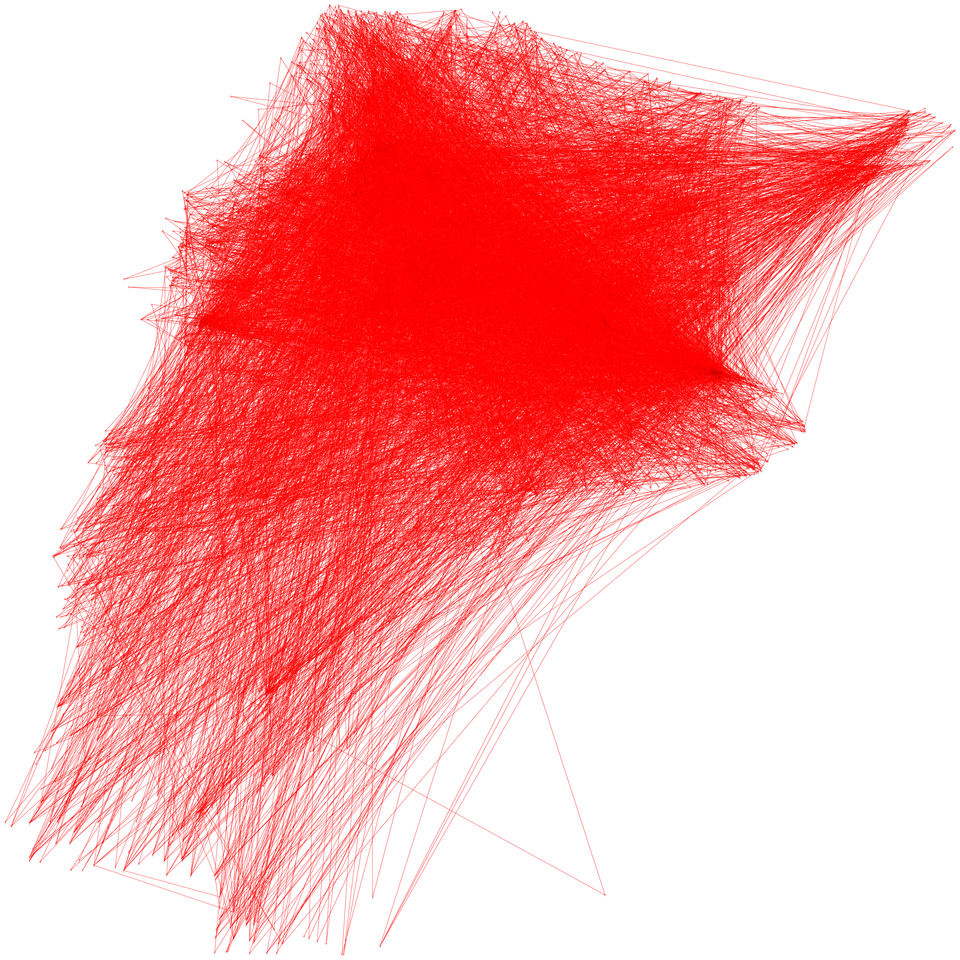
\includegraphics[width = 11cm,keepaspectratio]{img/output1}
		        \caption{Resultado utilizando o AG tradicional com 1 caixeiro.}
		        \label{tgat}
	   	\end{figure}
	   		
	   	\begin{figure}[h]
				\centering
		        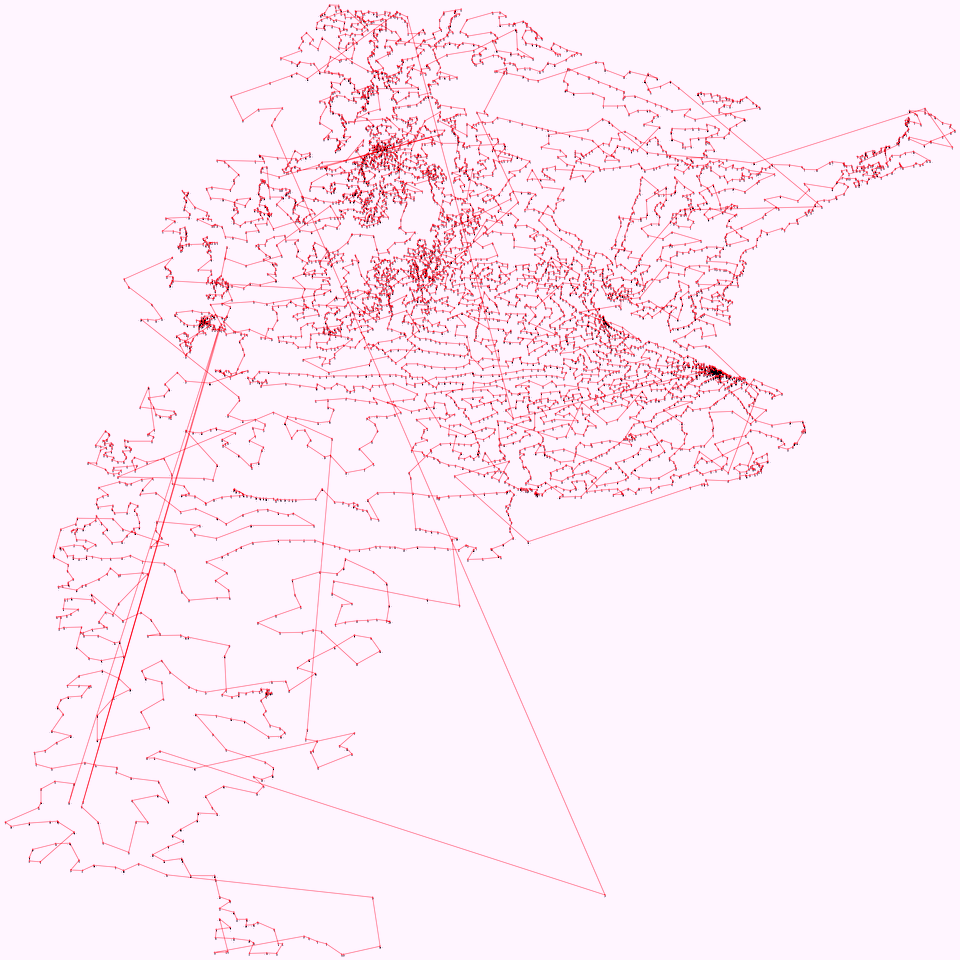
\includegraphics[width = 11cm,keepaspectratio]{img/output1n}
		        \caption{Resultado utilizando o AG híbrido  com 1 caixeiro.}
		        \label{tgan}
	   	\end{figure}
	   	
	   		\begin{figure}[h]
				\centering
		        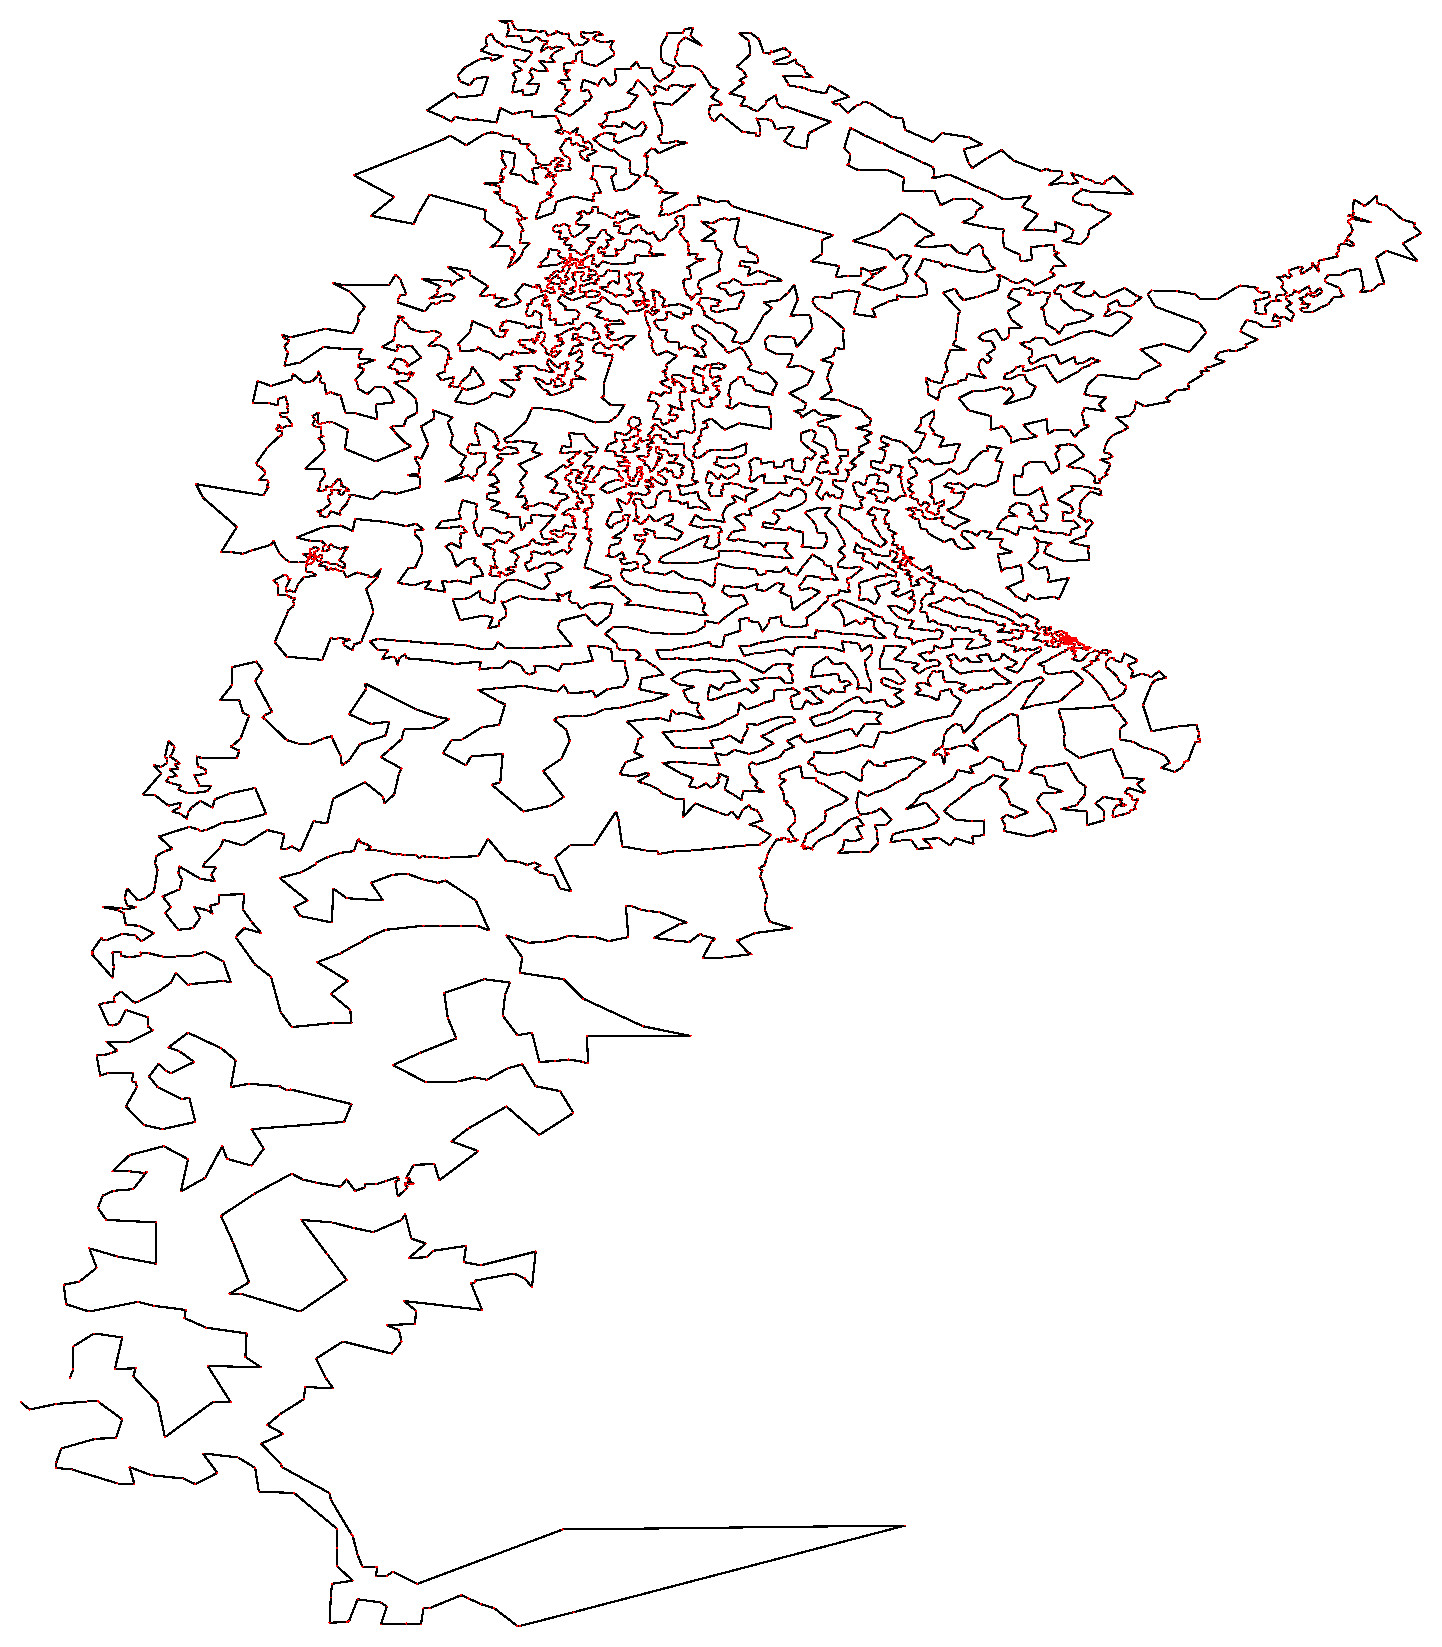
\includegraphics[width = 11cm,keepaspectratio]{img/artour}
		        \caption{Resultado TSPLIB.}
		        \caption*{Fonte: \cite{tsplib}}
		       
		        \label{arg}
	   	\end{figure}
	
		Também foram executados testes com 4 caixeiros viajantes. Os testes 3 (\textbf{figura~\ref{tgan4}}) e 4 (\textbf{figura~\ref{tga4}}) da \textbf{tabela~\ref{tab-t2}} demonstram que há uma grande diferença no tamanho das rotas geradas pelo Algoritmo Genético tradicional (73.338.600,00km) e o Algoritmo Genético Híbrido (1.145.840,00km).
		
		\begin{figure}[h]
				\centering
		        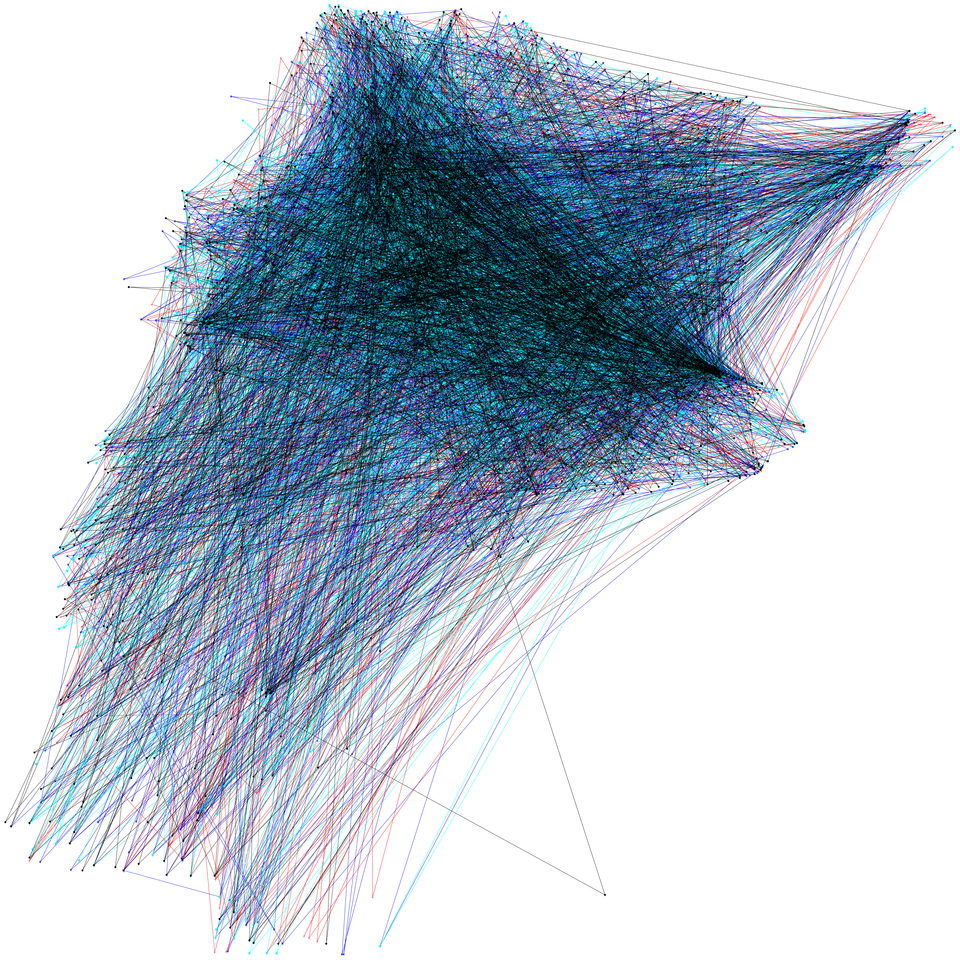
\includegraphics[width = 11cm,keepaspectratio]{img/output-4}
		        \caption{Resultado utilizando AG tradicional com 4 caixeiros (Argentina).}
		        \label{tga4}
	   	\end{figure}
	   		
	   	\begin{figure}[h]
				\centering
		        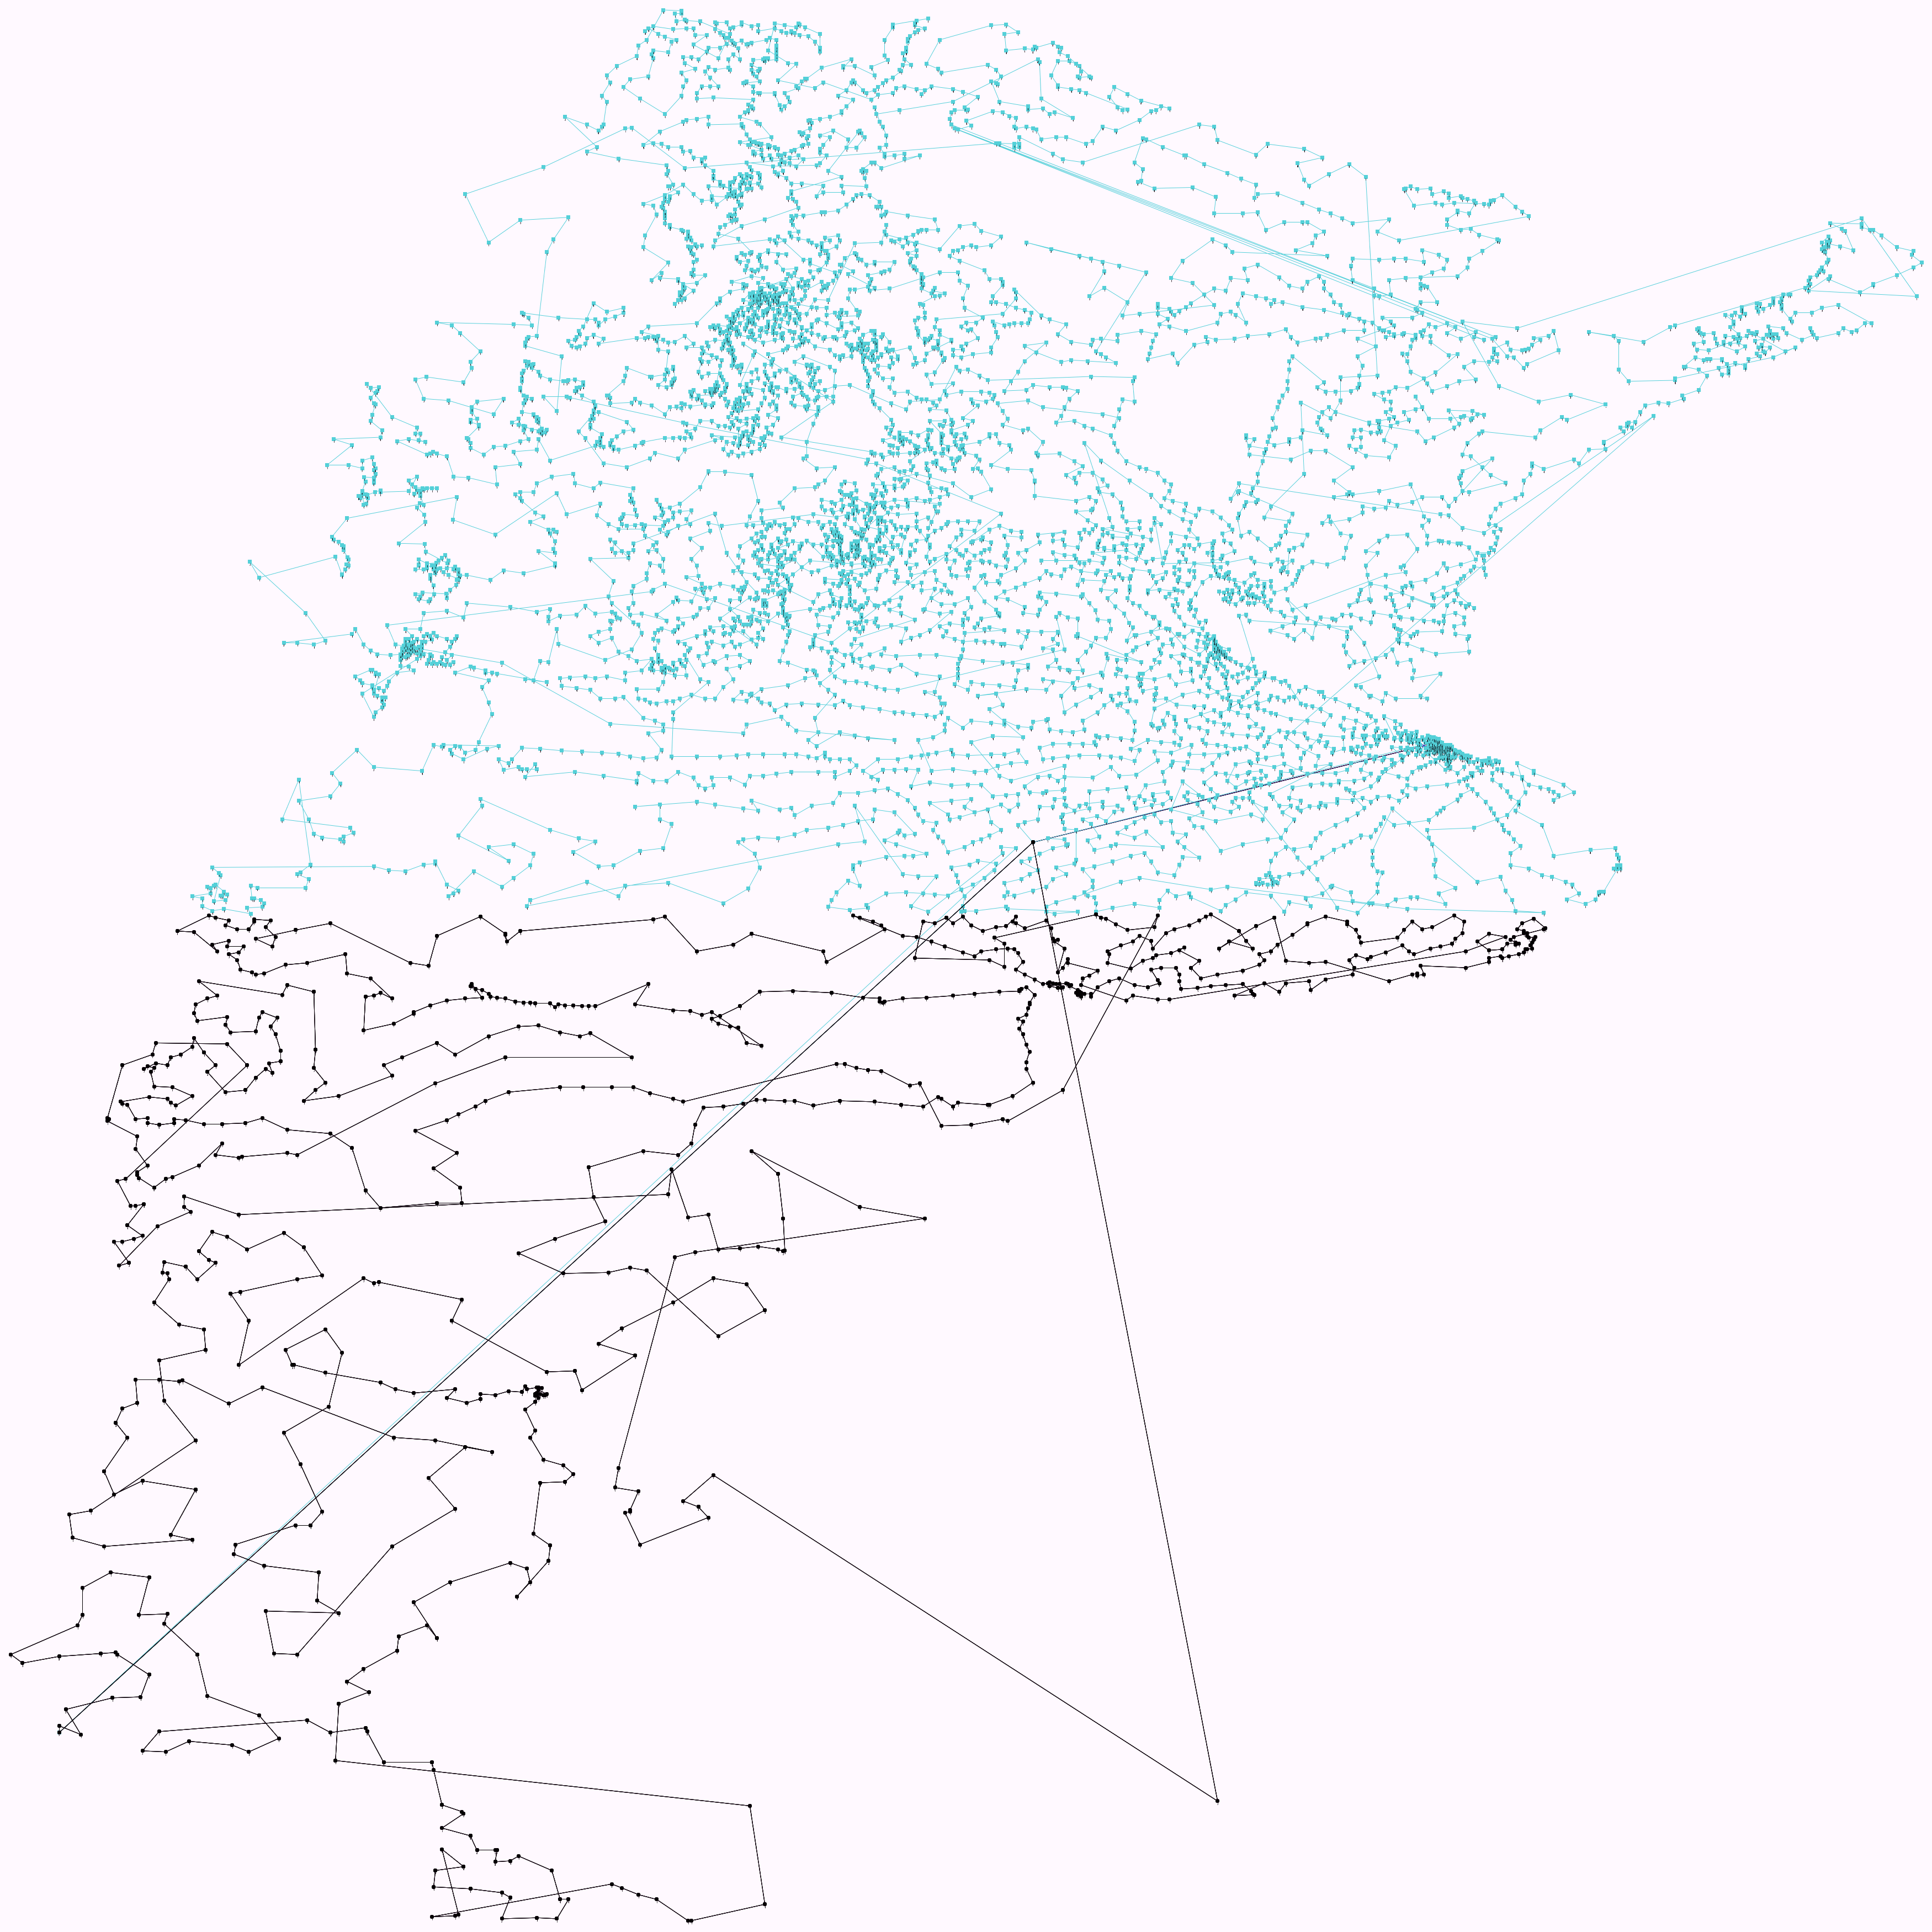
\includegraphics[width = 11cm,keepaspectratio]{img/output-nn-4}
		        \caption{Resultado utilizando AG Híbrido com 4 caixeiros (Argentina).}
		        \label{tgan4}
	   	\end{figure}
		
		\chapter{Conclusão}
		
	 Por meio desta pesquisa preliminar pode-se concluir que o Algoritmo Genético Híbrido desenvolvido é eficiente e economiza um tempo significativo de execução, mas ainda, não gera o resultado pretendido, pois suas rotas ainda são grandes comparadas com a base de teste \textit{TSPLIB}.
	 
	 O objetivo futuro é implementar diversos outros algoritmos para gerar a população inicial mais otimizada, já que o problema está neste, pois o indivíduo gerado pelo algoritmo \textit{Nearest-Neighbor} é muito superior à qualquer outro indivíduo gerado de forma aleatória, limitando a evolução da população, já que qualquer cruzamento entre estes indivíduos tem uma probabilidade remota de gerar um filho melhor que o indivíduo gerado pelo \textit{Nearest-Neighbor}.

%\begin{comment}
		%\section{Modelagem real}
		%\chapter{Conclusão}
%\end{comment}
	\bibliography{refs}

	\apendice
	\chapter{Código Fonte - main.cpp}
	\lstinputlisting{../code/algo_genetico_comum/agc/agc/main.cpp}
	\chapter{Código Fonte - ga.h}
	\lstinputlisting{../code/algo_genetico_comum/agc/agc/ga.h}
	\chapter{Código Fonte - ga.cpp}
	\lstinputlisting{../code/algo_genetico_comum/agc/agc/ga.cpp}

\end{document}
